\chapter{Diseño e implementación} 
\label{Chapter3} 

\section{Diseño de la arquitectura} 

\subsection{Propuestas de implementación} 

Durante el desarrollo del sistema se realizaron cuatro versiones principales, cada una marcando un cambio relevante en la tecnología, la arquitectura o el enfoque funcional del chatbot. A continuación, se describen cada una de estas iteraciones:

\subsubsection*{Versión 0 - RAG básico con Pinecone}

La necesidad inicial era construir un prototipo funcional para validar la arquitectura RAG utilizando herramientas accesibles.

\textbf{Descripción:} se implementó una arquitectura RAG elemental con una LLM (GPT-3.5-turbo) y el servicio de vectorstore Pinecone. El flujo básico consistía en preprocesar documentos, generar embeddings, almacenarlos en Pinecone y recuperar los chunks relevantes a partir de la pregunta del usuario con el objetivo de construir un prompt enriquecido que sería enviado a la LLM.

\textbf{Problemas detectados:} aunque Pinecone ofrecía un buen desempeño en la recuperación de información, su costo por consulta representaba un obstáculo considerable para su adopción en entornos de producción. Además, la trazabilidad del sistema era limitada, ya que no existían mecanismos para evaluar la calidad de los chunks obtenidos ni auditar el proceso de recuperación.

Esto puso de manifiesto la necesidad de un sistema de almacenamiento local que permitiera un mayor control sobre la generación, almacenamiento y recuperación de los embeddings. Asimismo, se requerían herramientas que facilitaran tanto la evaluación de las respuestas como la auditoría del flujo completo de recuperación de contextos reelevantes.

\subsubsection*{Versión 1 - Integración de DSPy, migración a LanceDB y uso de NemoGuardrails}
\textbf{Razón del cambio:} mejorar la calidad de las respuestas, reducir costos de infraestructura y establecer una capa de control conversacional previa a la ejecución del pipeline RAG.

\textbf{Descripción:} en esta versión se reemplazó Pinecone por LanceDB, una base de datos de vectores que permite almacenamiento local y ofrece mayor control sobre la estructura y acceso a los embeddings, eliminando costos asociados a servicios externos. 

Se integró DSPy, un framework que permite definir prompts de manera modular y declarativa, lo que facilitó una implementación más mantenible de la arquitectura RAG.

También se añadió una capa de filtrado con Nemo Guardrails para bloquear preguntas fuera de dominio, y un sistema de evaluación automática que puntuaba las respuestas del LLM, permitiendo monitorear su rendimiento. Estos componentes fueron implementados como módulos independientes en DSPy, mejorando la modularidad y claridad del sistema.

\begin{figure}[htbp]
    \centering
    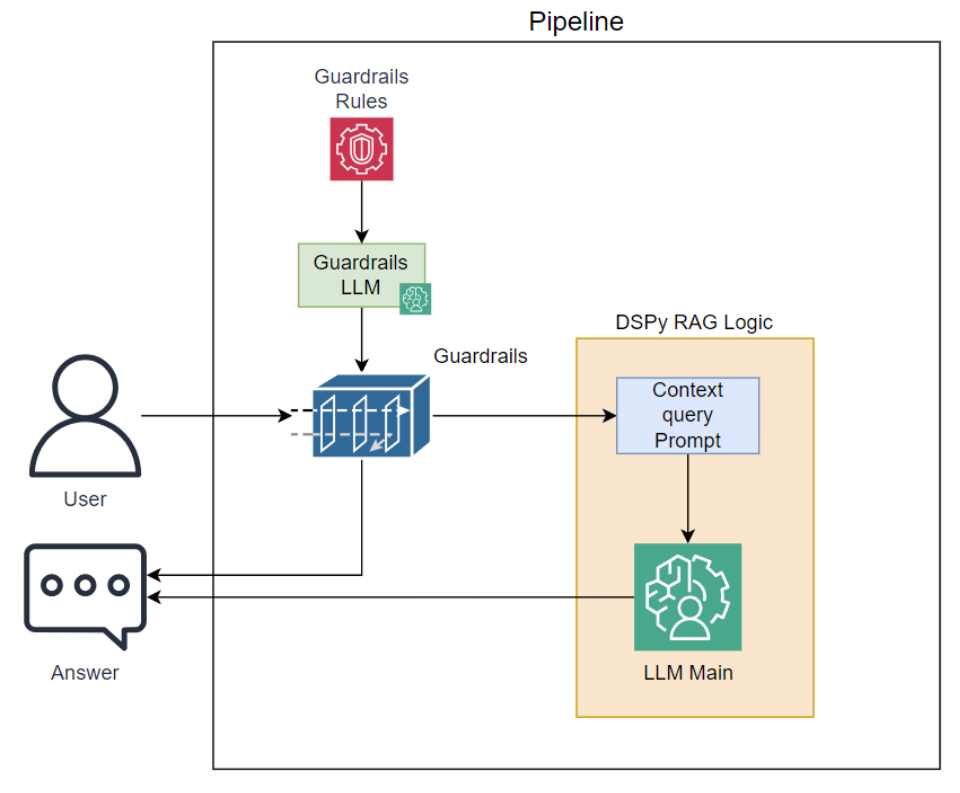
\includegraphics[width=.75\textwidth]{./Figures/version1.png}
    \caption{Diagrama general del sistema para la versión 1.}
    \label{fig:objetivos_venn}
  \end{figure}


\textbf{Problemas detectados:} aunque se logró una mayor robustez y control, surgieron varios desafíos. Nemo Guardrails mostró un rendimiento limitado en español y escasa capacidad de personalización, debido a su fuerte orientación al inglés, lo que redujo la eficacia del filtrado y motivó la búsqueda de alternativas más flexibles.

Además, si bien se incorporó un sistema de evaluación automática, aún no se contaba con trazabilidad completa de las interacciones ni con segmentación por métricas, aspectos que se abordarían en versiones posteriores.

\subsubsection*{Versión 2 - Guardrails personalizados, almacenamiento estructurado de chats e implementación del frontend y backend de pruebas}
\textbf{Razón del cambio:} necesidad de mayor precisión en el filtrado y mejor trazabilidad de las conversaciones.

\textbf{Descripción:} se reemplazó Nemo Guardrails por una implementación propia, basada en LLMs livianos y reglas personalizadas escritas en código con prompts propios, lo que permitió mayor flexibilidad y una mejor adaptación al idioma español. Además, se comenzó a almacenar localmente la conversación completa de cada usuario incluyendo preguntas, respuestas y contexto previo en la memoria RAM de manera local. Esto dotó al sistema de memoria conversacional, mejorando la coherencia de las respuestas y habilitando análisis posteriores sobre el historial de interacción. En paralelo, todas las interacciones del asistente (preguntas, respuestas, errores y rechazos por guardrails) comenzaron a registrarse en una base de datos NoSQL, lo que facilitó la trazabilidad de cada una de las interacciones de usuarios y el análisis detallado del comportamiento conversacional.

\begin{figure}[htbp]
    \centering
    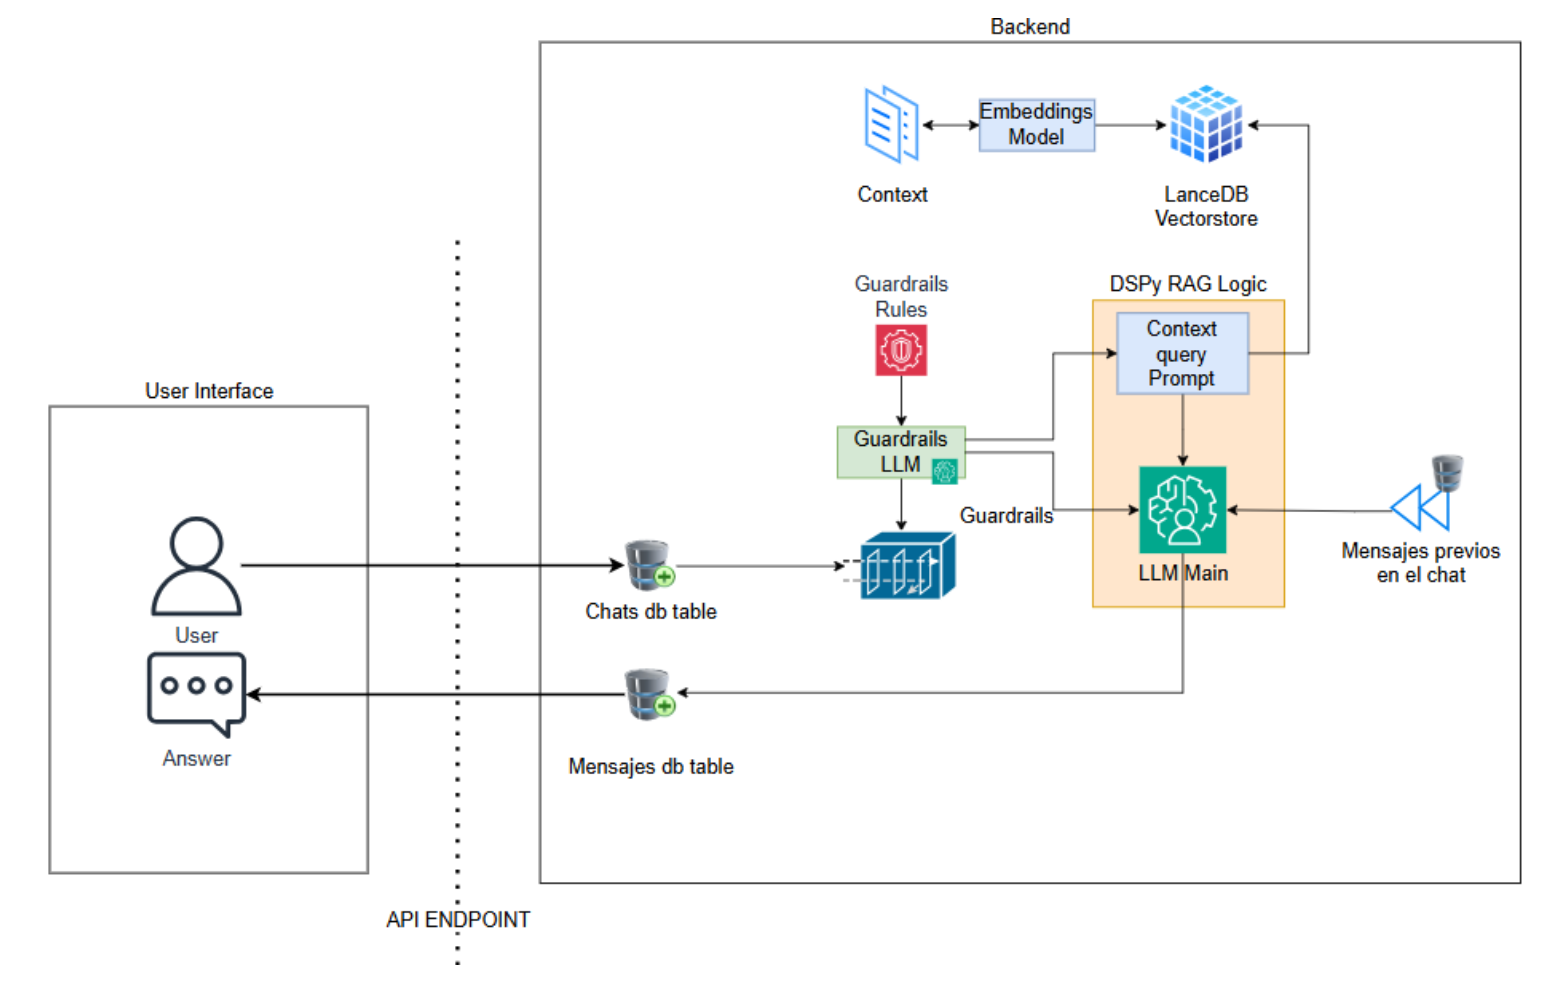
\includegraphics[width=.75\textwidth]{./Figures/version2.png}
    \caption{Diagrama general del sistema para la versión 2.}
    \label{fig:objetivos_venn}
  \end{figure}

\textbf{Problemas detectados:} aunque el nuevo sistema de guardrails ofreció mayor control, la forma en la que se persistian los historiales de conversación generó un aumento significativo en el uso de memoria RAM, lo que limitó la escalabilidad del sistema. Además, la latencia de respuesta aumentó considerablemente, lo que afectó la experiencia del usuario. Por último, si bien el almacenamiento de las conversaciones facilitó el contexto en interacciones encadenadas, se detectó que para casos en los que la pregunta dependía de la pregunta anterior, los contextos no eran claros. Ejemplo:

\begin{itemize}
    \item Usuario: "¿Tienen Stock del producto X?"
    \item Robot: "Sí, tenemos stock del producto X."
    \item Usuario: "¿Cuánto cuesta?"
    \item Robot: "Podrías aclarar de qué producto hablas?"
\end{itemize}

En este caso, el sistema no pudo identificar que la pregunta se refería al producto mencionado en la pregunta anterior. Esto evidenció la necesidad de un sistema de redefinición de preguntas que pudiera enriquecer el contexto y mejorar la recuperación de información utilizando palabras clave que referencien el contexto de la conversación.


\subsubsection*{Versión 3 - Integración de Langfuse, clasificación y evaluación automática}
\textbf{Razón del cambio:} necesidad de un sistema robusto para trazabilidad, evaluación y mejora continua.

\textbf{Descripción:} se integró Langfuse como sistema observador no intrusivo para registrar todas las interacciones del sistema. además, se añadieron dos nuevas tareas en la capa de guardrails: la primera, redefinir preguntas, genera una nueva oración con palabras clave para buscar los contextos en la vectorestore; la segunda tarea, clasificar consultas, organiza las preguntas según su temática, como por ejemplo Productos, Precios, Delivery, Queja, Saludo, entre otras. También se eliminaron bases de datos auxiliares, centralizando la gestión de la trazabilidad en Langfuse, que ahora se encarga de registrar todos los eventos: consultas, respuestas, errores, rechazos por guardrails, consumo de tokens, costos, latencia, etc.



\begin{figure}[htbp]
    \centering
    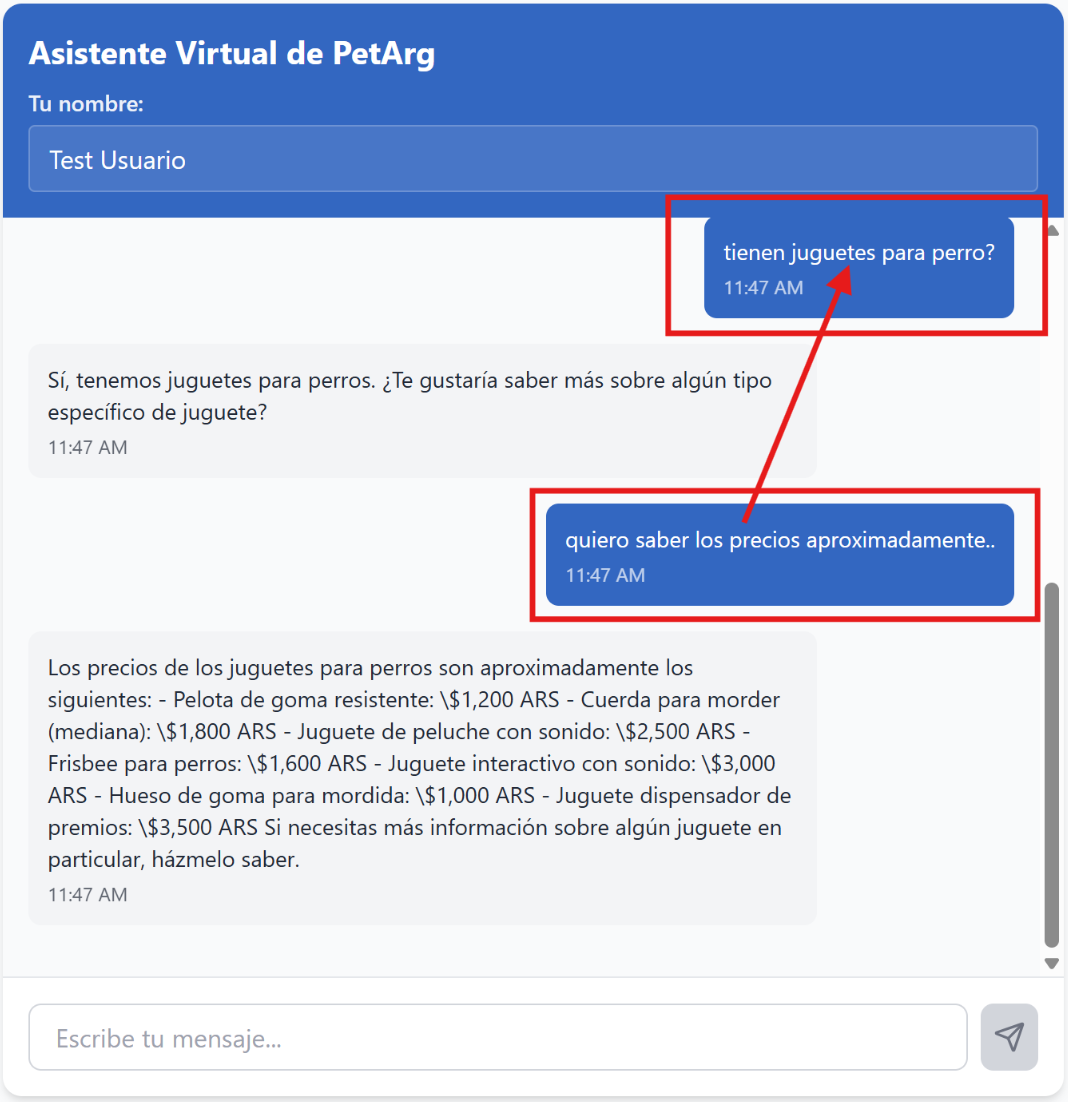
\includegraphics[width=.75\textwidth]{./Figures/ejemploreformulado.png}
    \caption{Ejemplo de redefinición de pregunta.}
    \label{fig:objetivos_venn}
  \end{figure}

\textbf{Problemas detectados:} algunos temas, como las quejas, mostraron un rendimiento inferior, lo que sugiere la necesidad de expandir y refinar el contexto disponible en versiones futuras.


\subsection{Problemas y mitigaciones} 

Durante las primeras iteraciones surgieron limitaciones clave: costos por servicios externos (Pinecone, API de LLMs), pobre trazabilidad del sistema, y ausencia de control sobre la evaluación de calidad. Estos problemas se mitigaron mediante:

\begin{itemize}
    \item \textbf{Migración a LanceDB para almacenamiento local sin costo.} LanceDB es una base de datos vectorial optimizada para uso local. Su adopción permitió eliminar la dependencia de servicios como Pinecone, que implicaban costos por cada consulta. Esta decisión fue especialmente útil durante la etapa de desarrollo y pruebas, ya que redujo los costos operativos. Sin embargo, se observó que LanceDB puede presentar latencias más altas en comparación con soluciones SaaS (software as a service), lo cual debe considerarse en entornos de producción. Por otra parte, para aplicaciones a gran escala, su uso local podría representar un ahorro sustancial al evitar tarifas por tokens o uso de APIs externas.

    \item \textbf{Uso de DSPy para estructurar la lógica RAG y mejorar la modularidad.} DSPy es una biblioteca que permite construir y optimizar pipelines de IA mediante una programación declarativa. Se utilizó para implementar de manera modular el sistema RAG, definiendo claramente etapas de recuperación y generación. Esta implementación facilitó la trazabilidad del proceso completo, permitiendo auditar tanto la recuperación de contextos como la generación de respuestas. Además, su enfoque declarativo simplificó el desarrollo, mejorando la mantenibilidad y facilitando la introducción de mejoras incrementales al sistema.

    \item \textbf{Reemplazo de Nemo Guardrails por guardrails personalizados.} NeMo Guardrails no ofrecía resultados adecuados para preguntas en español. Por este motivo, se diseñó una solución propia basada en prompts simples con modelos LLM. Esta implementación personalizada fue capaz de detectar y filtrar preguntas sobre política, religión y temas sensibles. Además, se utilizó como etapa inicial para la clasificación temática y la redefinición de preguntas en etapas posteriores.

    \item \textbf{Incorporación de Langfuse como observador centralizado y sistema de métricas.} Langfuse es una herramienta de observabilidad que permite registrar, analizar y etiquetar cada interacción con el modelo. Su integración aportó trazabilidad completa del sistema, facilitó el monitoreo de métricas clave (como latencia, consumo de tokens, respuestas generadas) y habilitó la evaluación automática mediante la implementación de agentes de evaluación con IA en su plataforma. Gracias a esta integración, se logró una visión integral del rendimiento del sistema, permitiendo identificar áreas de mejora y optimizar el flujo de trabajo. Gracias a esta capacidad, se procedió a eliminar la etapa de DSPy que se encargaba de la evaluación automática, posterior a la respuesta de la LLM. Esto disminuyó la latencia del sistema y permitió una mejor trazabilidad de las interacciones, ya que Langfuse almacena todos los eventos generados por el sistema, incluyendo la evaluación automática. Esto permite auditar el funcionamiento del sistema y mejorar el contexto disponible en la etapa de analisis de métricas.
\end{itemize}


\subsection{Elección de la arquitectura de chatbot} 

La arquitectura final del chatbot se fundamenta en el enfoque RAG (Retrieval-Augmented Generation), una técnica que ha demostrado ser altamente efectiva para responder preguntas contextualizadas sin necesidad de realizar un reentrenamiento completo del modelo de lenguaje (LLM). Esta decisión se basó en la necesidad de ofrecer un sistema flexible, escalable y de bajo costo operativo, especialmente orientado a pequeñas empresas y emprendedores que requieren soluciones ágiles y sostenibles.

El uso de RAG permite mantener el modelo LLM independiente de la base de conocimiento, lo que significa que se pueden incorporar nuevos documentos, actualizaciones o correcciones simplemente modificando los datos almacenados en el vectorstore, sin necesidad de ajustar los parámetros del modelo. Esta separación entre el modelo y la información facilita enormemente las tareas de mantenimiento y mejora continua del sistema.

Esta arquitectura RAG se seleccionó por ofrecer un equilibrio óptimo entre precisión, costo y mantenibilidad. Durante el desarrollo del proyecto, OpenAI lanzó GPT-4o mini, un modelo que presentaba un excelente balance entre rendimiento y economía, con capacidades superiores a las alternativas locales disponibles en ese momento. Si bien se evaluó la posibilidad de implementar un modelo local con Ollama, la combinación de GPT-4o mini con LanceDB resultó ser más eficiente en términos de costo-beneficio, ya que eliminaba la necesidad de infraestructura adicional para hospedar y mantener modelos locales. Esta decisión permitió reducir significativamente el costo por consulta mientras se mantenía un alto estándar de calidad en las respuestas, haciendo que la solución fuera más accesible para pequeñas empresas y emprendedores. Adicionalmente, el uso de componentes modulares como DSPy facilitó que el sistema pudiera adaptarse fácilmente a nuevos modelos o proveedores de LLMs en el futuro, sin necesidad de rediseñar toda la arquitectura.


\section{Arquitectura final propuesta} 

La arquitectura final del sistema está diseñada para ofrecer una solución robusta, eficiente y fácilmente escalable para la automatización de respuestas contextuales. Está compuesta por los siguientes bloques funcionales:

\begin{itemize}
    \item \textbf{Frontend}: interfaz renovada para usuarios y administradores. Permite enviar preguntas al sistema, visualizar respuestas, acceder a métricas y gestionar los contextos mediante un formulario ilustrativo.
    \begin{figure}[htbp]
        \centering
        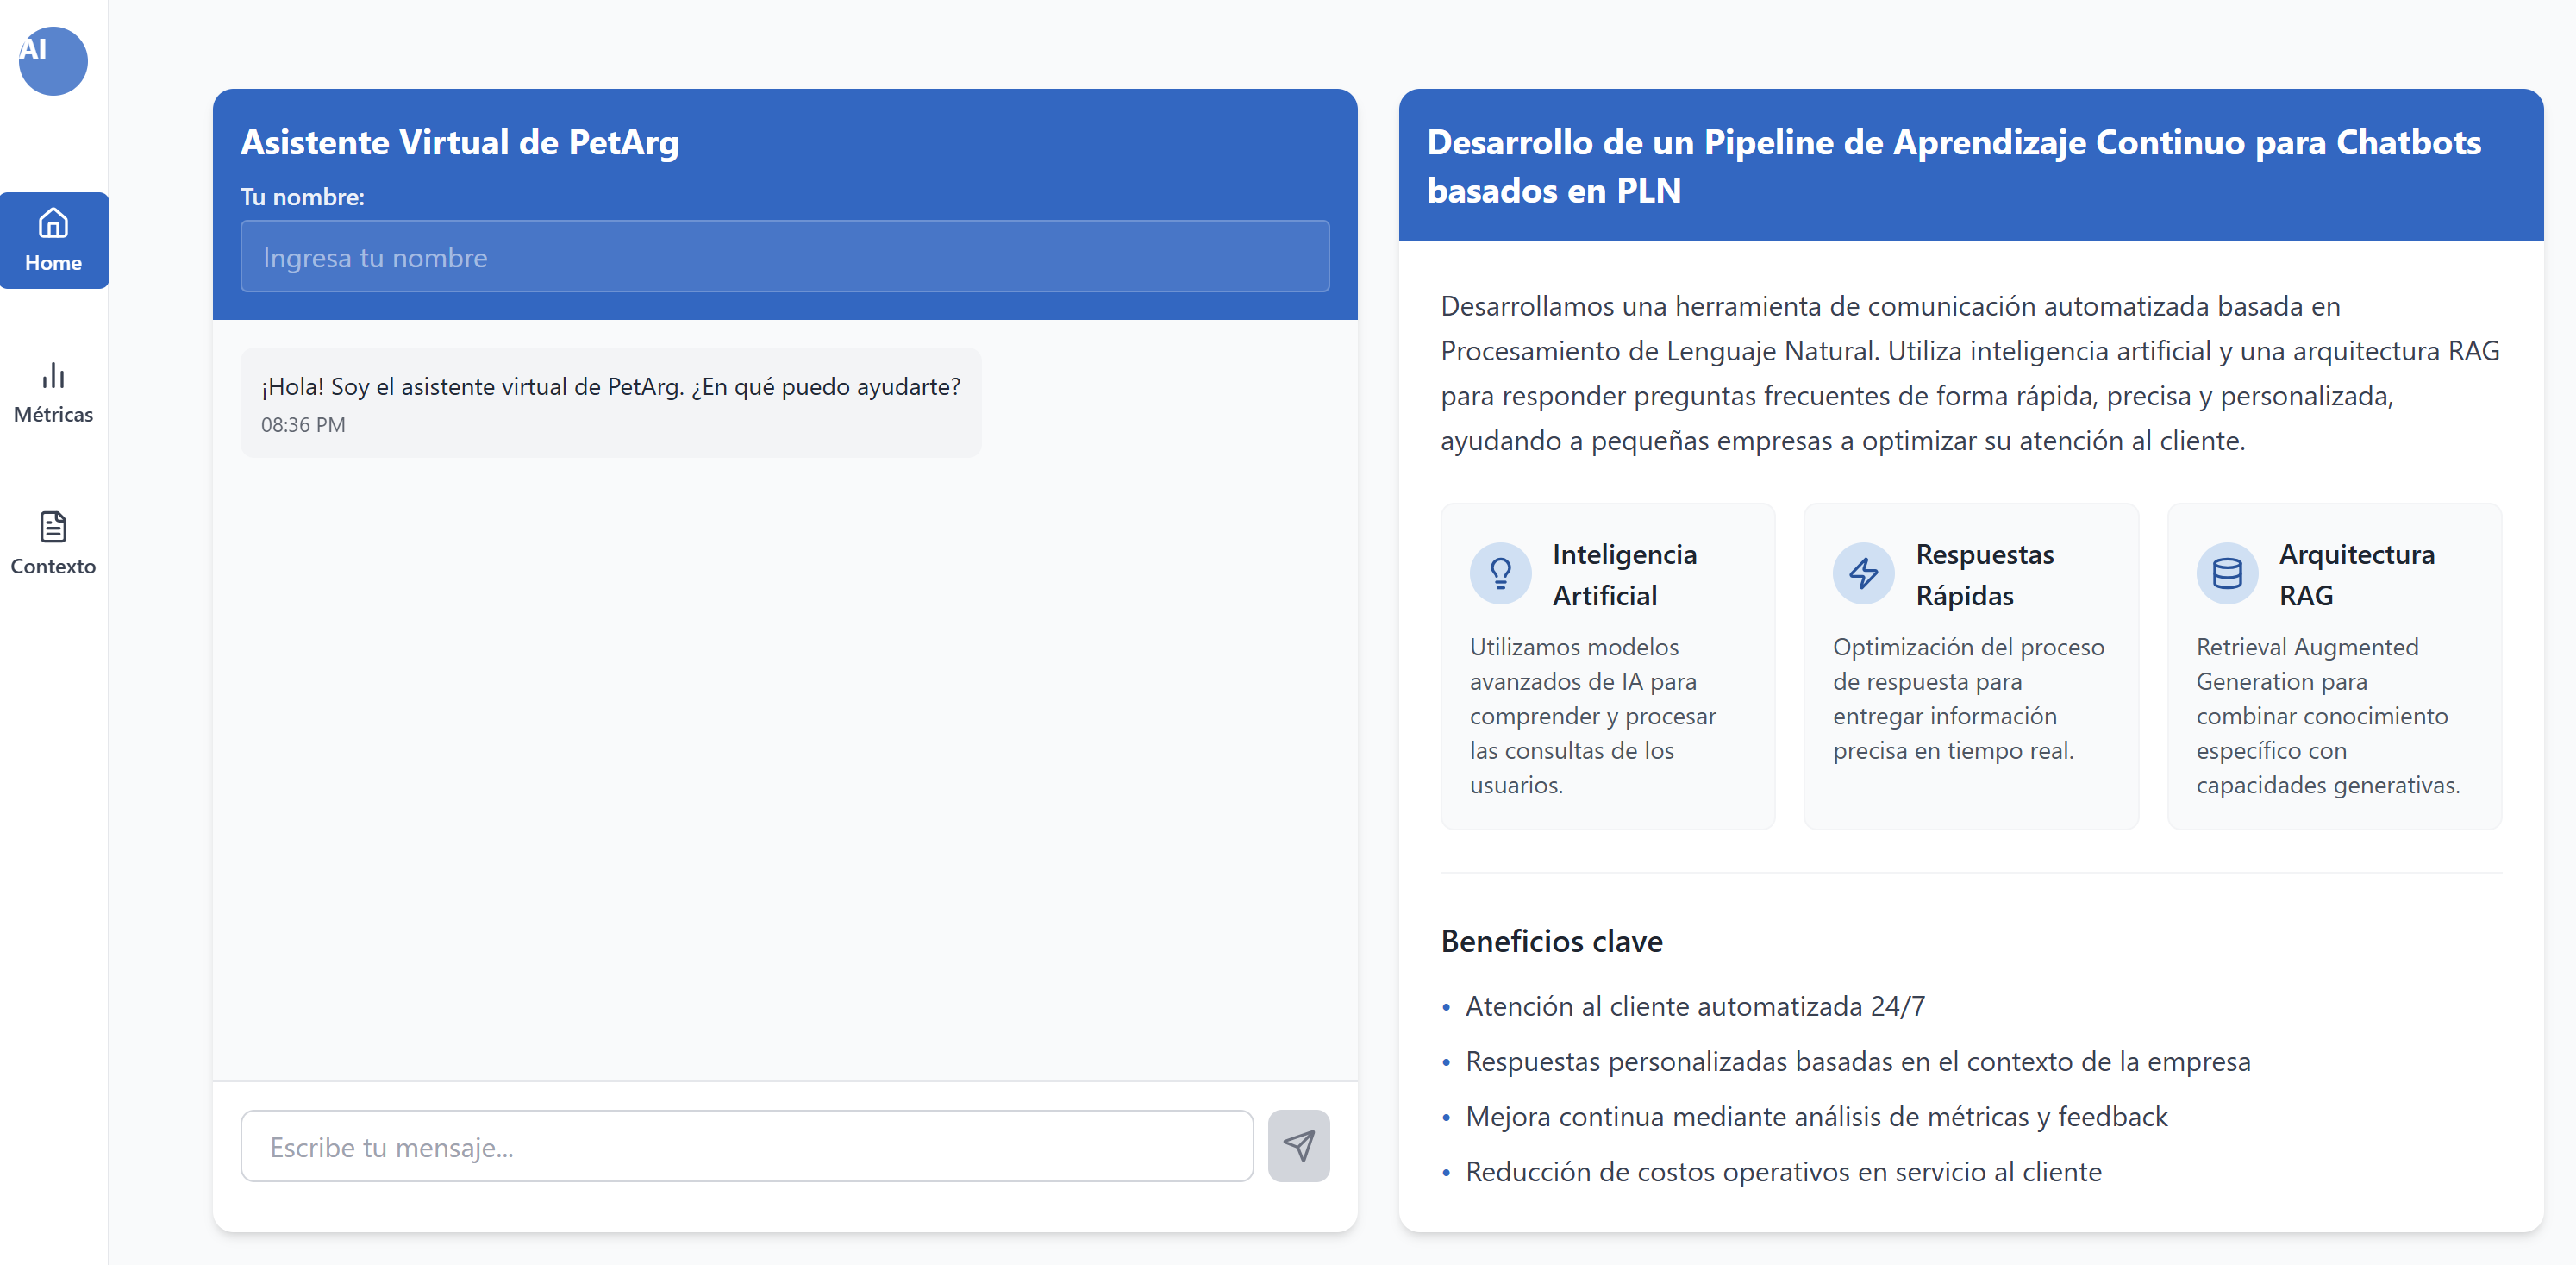
\includegraphics[width=.75\textwidth]{./Figures/frontend.png}
        \caption{Frontend del chatbot.}
        \label{fig:objetivos_venn}
      \end{figure}

    \item \textbf{Backend}: implementado en FastAPI, se encarga de recibir los request del frontend para procesar las preguntas, enviar las respuestas, procesar las métricas requeridas y actualizar los contextos en la base de datos de vectores. Gestiona el flujo completo de la conversación, registrando cada interacción, clasificando temáticamente las preguntas, redefiniéndolas usando el historial de mensajes previos, y preparando la consulta para la lógica RAG. Además, se encarga de procesar las métricas leyendo las trazas de Langfuse, analizando patrones de uso, calculando estadísticas de rendimiento y enviando estos análisis al frontend para que este los ilustre mediante gráficos y dashboards interactivos, facilitando así la visualización de tendencias y áreas de mejora del sistema.
    
    \item \textbf{Guardrails}: módulo de filtrado y preprocesamiento que evalúa si una consulta es válida (según reglas predefinidas), la clasifica en categorías como "Producto", "Quejas", "Saludos"; y la redefine incorporando el contexto de los mensajes anteriores.
    
    \item \textbf{DSPy RAG}: es el corazón del sistema, responsable de orquestar la lógica principal del flujo RAG. DSPy toma la pregunta ya enriquecida desde el módulo de guardrails y ejecuta una búsqueda eficiente de contextos relevantes en LanceDB. A partir de los fragmentos recuperados, construye un prompt enriquecido que será enviado al modelo LLM para generar una respuesta coherente y precisa. Además de facilitar la integración de prompts, DSPy permite definir y estructurar toda la lógica del sistema de recuperación y generación, proporcionando un marco flexible y modular para el diseño del flujo completo.
    
    \item \textbf{Langfuse}: observador pasivo que registra todas las interacciones del sistema sin intervenir. Almacena información crítica como la pregunta original, la redefinida, el consumo de tokens, la respuesta final y los estados de los guardrails. También permite aplicar evaluaciones automáticas sobre precisión de las respuestas generadas por el sistema.
\end{itemize}

\begin{figure}[htbp]
    \centering
    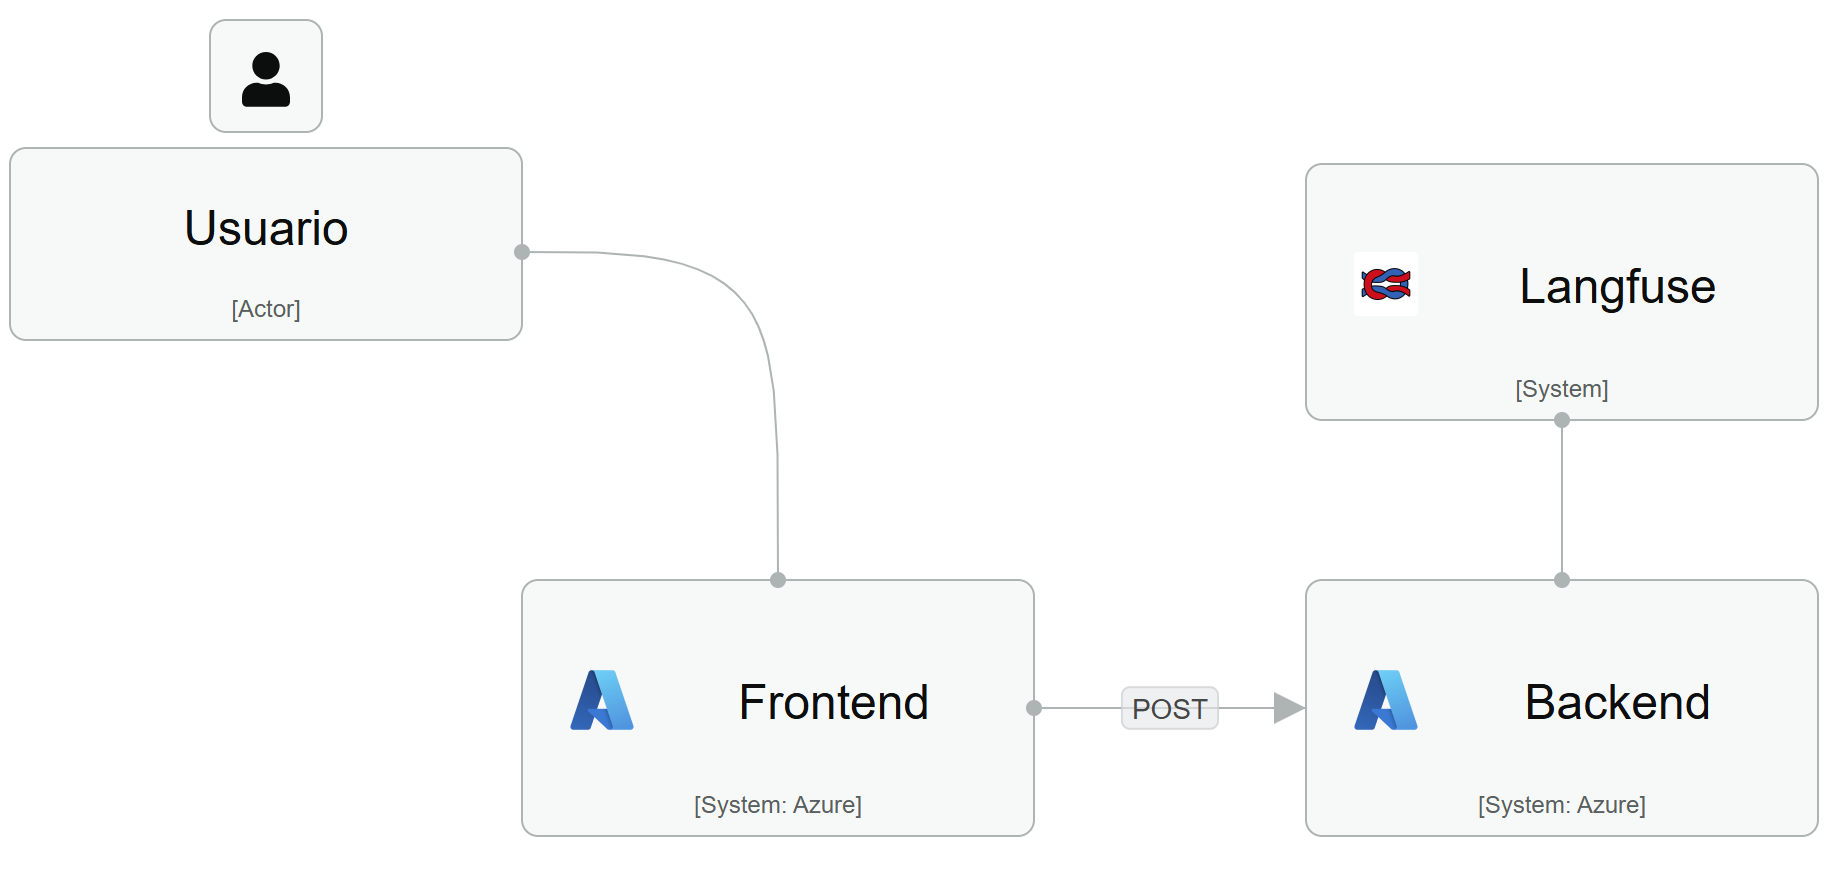
\includegraphics[width=.75\textwidth]{./Figures/highlevel.png}
    \caption{Diagrama general del flujo del pipeline.}
    \label{fig:objetivos_venn}
\end{figure}

\subsection{Tecnologías suplementarias} 

\begin{itemize}
    \item \textbf{Streamlit}: utilizado para construir el frontend inicial de pruebas, permitiendo interacción simple del chat, que luego fue migrada a ReactJS.

    \item \textbf{Lovable}:  lovable.dev es una herramienta online que permite crear frontends de forma rápida y sencilla con la ayuda de Inteligencia Artificial. Fue utilizada para crear la version final del frontend utilizando ReactJS, permitiendo una experiencia de usuario más fluida y atractiva. Además en ella se integraron las visualizaciones de las métricas generadas a partir de los datos de Langfuse.

    \item \textbf{Azure Container Apps}: Plataforma de Azure utilizada para desplegar el backend y el frontend del sistema en containers individuales. Permite escalar automáticamente los recursos según la demanda, asegurando un rendimiento óptimo en todo momento.
\end{itemize}

\subsection{Funcionamiento general} 

El pipeline del sistema está diseñado para ofrecer una experiencia conversacional precisa, eficiente y trazable. A continuación se detalla el flujo completo de funcionamiento desde la perspectiva funcional:


\begin{enumerate}
    \item El usuario realiza una consulta a través del \textbf{frontend}.
    
    \item La consulta es enviada al \textbf{backend}, donde primero pasa por un sistema de \textbf{guardrails personalizados}. Aquí se ejecutan tres procesos clave:
    \begin{itemize}
        \item \textbf{Filtrado}: se descartan preguntas fuera del dominio del sistema (por ejemplo, política o religión), basándose en reglas definidas.
        \item \textbf{Clasificación}: la pregunta se categoriza automáticamente en una temática (Producto, Quejas, Saludos, etc.).
        \item \textbf{Redefinición}: utilizando el historial conversacional completo, la pregunta se reformula para enriquecer su significado y contexto.
    \end{itemize}
    
    \item La pregunta redefinida es ingresada al primer modulo de DSPy donde es utilizada para buscar en \textbf{LanceDB}, los fragmentos de contexto indexados previamente que estan relacionados a la pregunta en cuestion.
    
    \item La información obtenida se utiliza para construir un \textbf{prompt estructurado en el siguiente modulo de DSPy}. Esta es la etapa lógica mas importante del pipeline ya que aqui se encuentra el corazon del sistema RAG, en esta etapa es donde se integra tanto el contexto recuperado como la consulta original para preparar la entrada final al LLM.
    
    \item El prompt es enviado a un \textbf{modelo LLM} (en este caso GPT-4o mini).
    
    \item La respuesta y todos los datos asociados (estado del guardrail, redefinición, tokens consumidos, clasificación, etc.) son registrados por \textbf{Langfuse}.
    
    \item En Langfuse, se ejecuta una \textbf{evaluación automática}, la cual analiza la calidad y asigna puntajes en una escala de 1 a 10, donde las puntuaciones bajas  (menores a 3) indican respuestas que solo reformulan la pregunta o evidencian insuficiencia de contexto. Los criterios de evaluación son:
        \begin{itemize}
            \item \textbf{Precisión}: determina si la respuesta aborda directamente la pregunta del usuario o simplemente la reformula sin proporcionar información sustancial.
            \item \textbf{Suficiencia de contexto}: evalúa si la respuesta demuestra que el sistema disponía de información adecuada para contestar con propiedad o si indica explícitamente la falta de contexto necesario.
        \end{itemize}
        
        
    \item En paralelo con la observación de Langfuse, la respuesta es devuelta al usuario en el frontend.
\end{enumerate}

\begin{figure}[htbp]
    \centering
    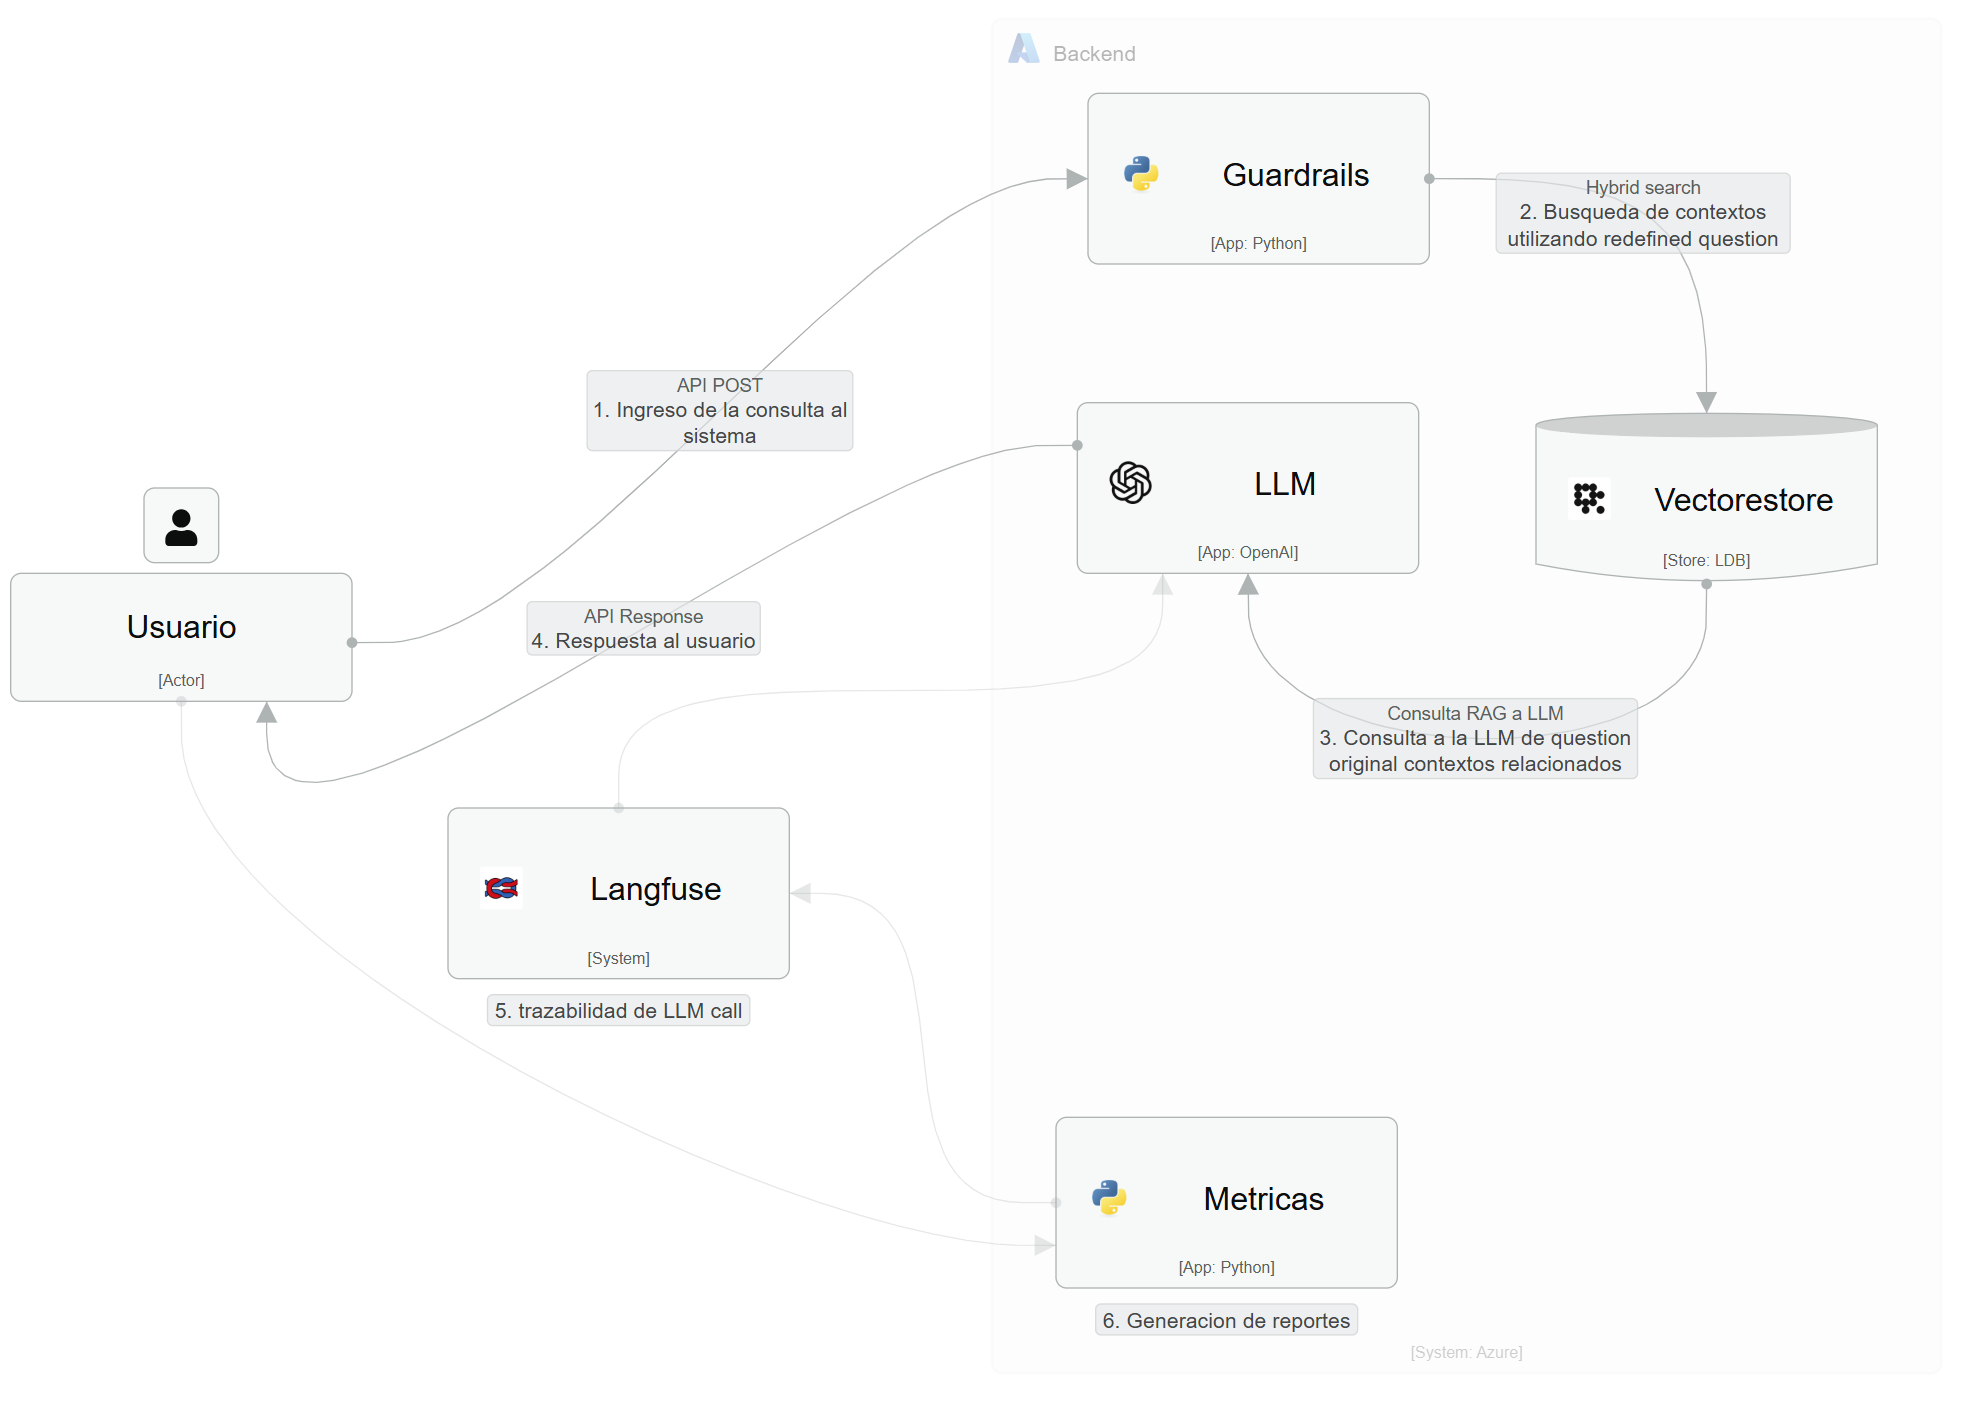
\includegraphics[width=.75\textwidth]{./Figures/svgtech.png}
    \caption{Diagrama de flujo de funcionamiento.}
    \label{fig:objetivos_venn}
\end{figure}


% new page 

\newpage
\section{Implementación} 

  \subsection{Preparación de los datos de contexto} 
  
  La base de conocimiento utilizada por el sistema no proviene de documentos extensos procesados en chunks, sino de una estructura de tipo clave-valor diseñada específicamente para búsquedas contextuales rápidas y precisas. Cada entrada contiene dos campos principales:
  
  \begin{itemize}
      \item \textbf{question}: una lista de términos, sinónimos o expresiones relacionadas que representan la intención del usuario. este campo actúa como una clave semántica para la búsqueda.
      \item \textbf{relates}: una serie de frases informativas asociadas a la clave, que constituyen el contexto que será devuelto al modelo como parte del proceso RAG.
  \end{itemize}

  \begin{lstlisting}[language=Python, caption={Ejemplo de estructura de datos clave-valor para el contexto}]
    context = [
        {
            question: [
                queja,
                reclamo,
                problema],

            relates: [
                Lamentamos que hayas tenido una mala
                experiencia. Por favor cuentanos mas
                sobre tu situacion, Estamos aqui
                para ayudarte con cualquier
                inconveniente que hayas tenido
            ]
        },
        {
            question: [
                producto, 
                caracteristicas, 
                especificaciones],

            relates: [
                Nuestro producto cuenta 
                con las siguientes caracteristicas,
                Las especificaciones tecnicas son
            ]
        }
    ]   
    \end{lstlisting}
    
    
  Durante la interacción, el sistema utiliza un LLM para reformular la consulta del usuario e identificar las claves más relevantes, luego estas keywords son utilizadas por LanceDB para ser comparadas con el conjunto \texttt{question}. A partir de esta coincidencia semántica y vectorial (la busqueda es hybrida), se recuperan los valores correspondientes desde el campo \texttt{relates}, que son luego inyectados como contexto en el prompt del LLM generador.
  

  \subsection{Sistema de reentrenamiento con historiales y evaluación automatizada de interacciones}
  
  A lo largo del desarrollo del sistema, se adoptó un enfoque alternativo al reentrenamiento tradicional de modelos de lenguaje (LLM), priorizando la adaptabilidad continua mediante mecanismos de evaluación automática y actualización contextual. Esta arquitectura permite que el sistema analice los resultados de las interacciones con los usuarios sin modificar directamente los parámetros internos del modelo base.

  En lugar de reentrenar el LLM, se mantiene un ciclo de mejora continua alimentado por datos conversacionales reales. Estos datos son organizados, evaluados y analizados a través de herramientas automatizadas. El administrador es responsable de revisar las métricas generadas y decidir si es necesario realizar ajustes en el sistema, gestionando los contextos almacenados en la base de datos vectorial LanceDB, a través del frontend en la interfaz de administración.
  

\vspace{1em}
\noindent
\begin{figure}[htbp]
    \centering
    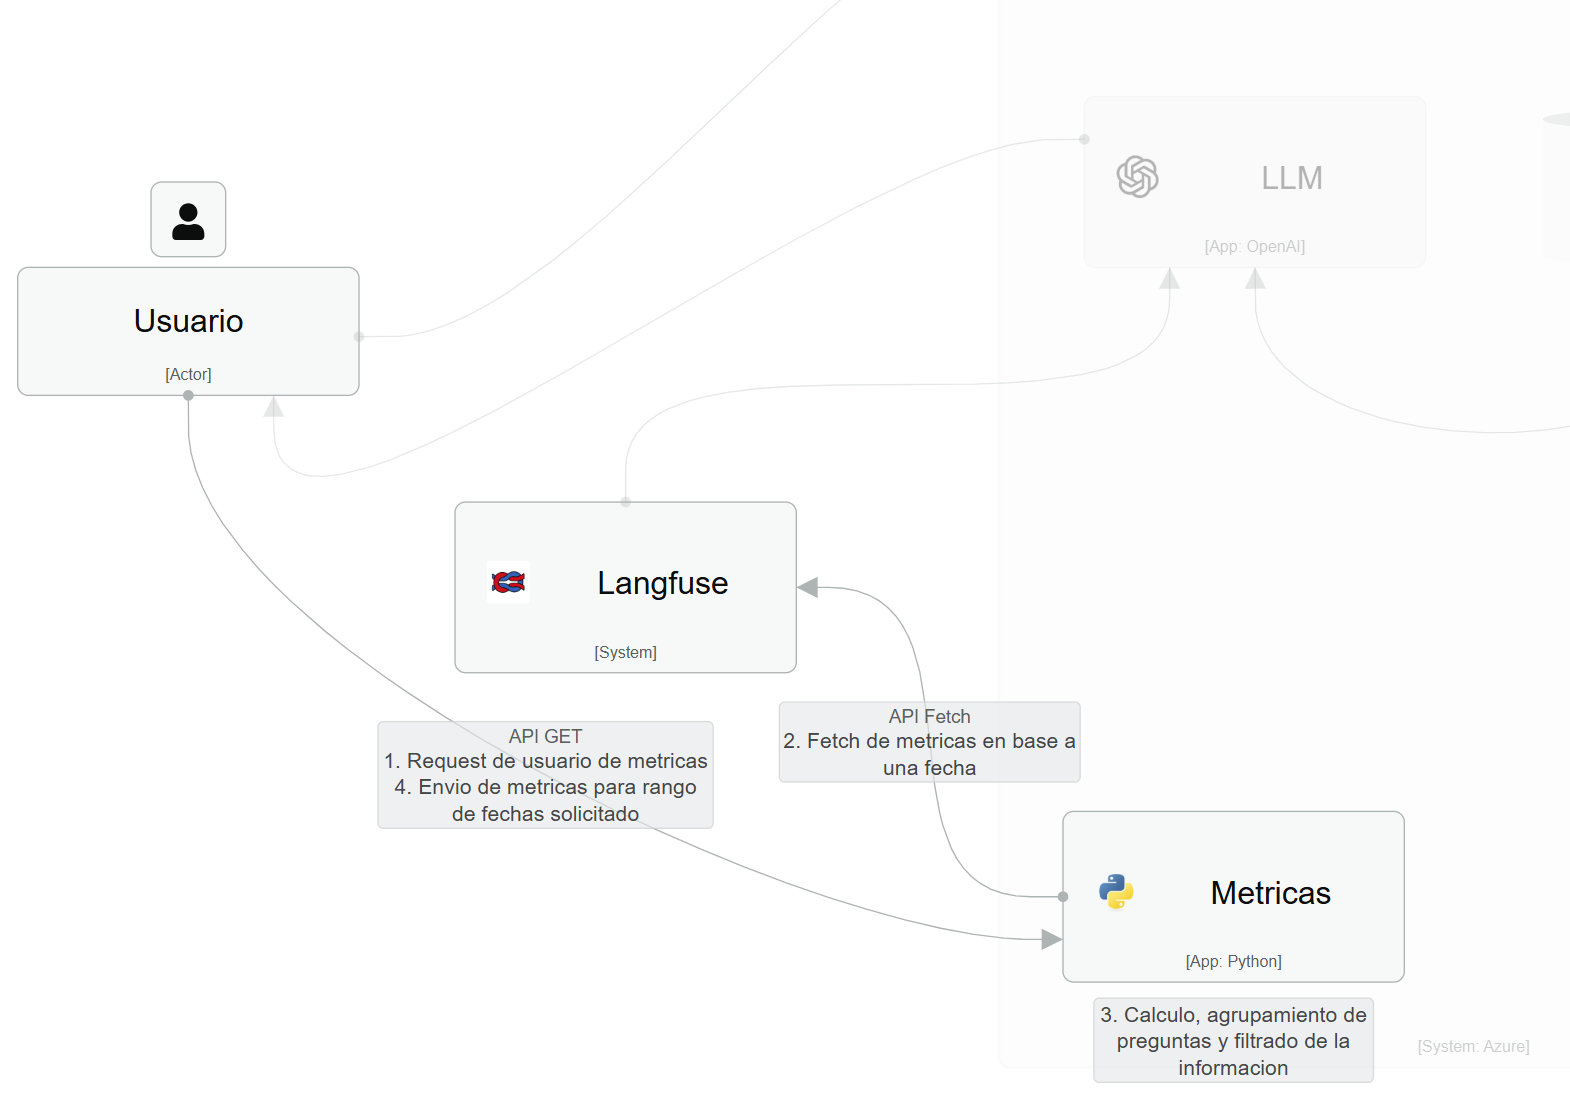
\includegraphics[width=.75\textwidth]{./Figures/flujometricas.png}
    \caption{Diagrama de flujo de observación de métricas.}
    \label{fig:objetivos_venn}
  \end{figure}


\subsubsection*{Evaluación automatizada y extracción de métricas}

Cada interacción registrada en el sistema genera una “traza” que es almacenada mediante Langfuse. Estas trazas contienen no solo los mensajes de entrada y salida, sino también metainformación crucial: costo (tokens consumidos y dinero gastado), etiquetas temáticas (por dominio o tipo de consulta), comentarios evaluativos y puntajes de calidad (en una escala del 1 al 10).

Las evaluaciones son gestionadas por un proceso automatizado que recorre todas las trazas válidas (excluyendo categorías genéricas como "Saludo" u "Otros"), e identifica aquellas que contienen puntuaciones explícitas (`trace.scores`). El código utilizado implementa un control de tasa (rate limit) y asegura la integridad del dataset.

\begin{figure}[htbp]
    \centering
    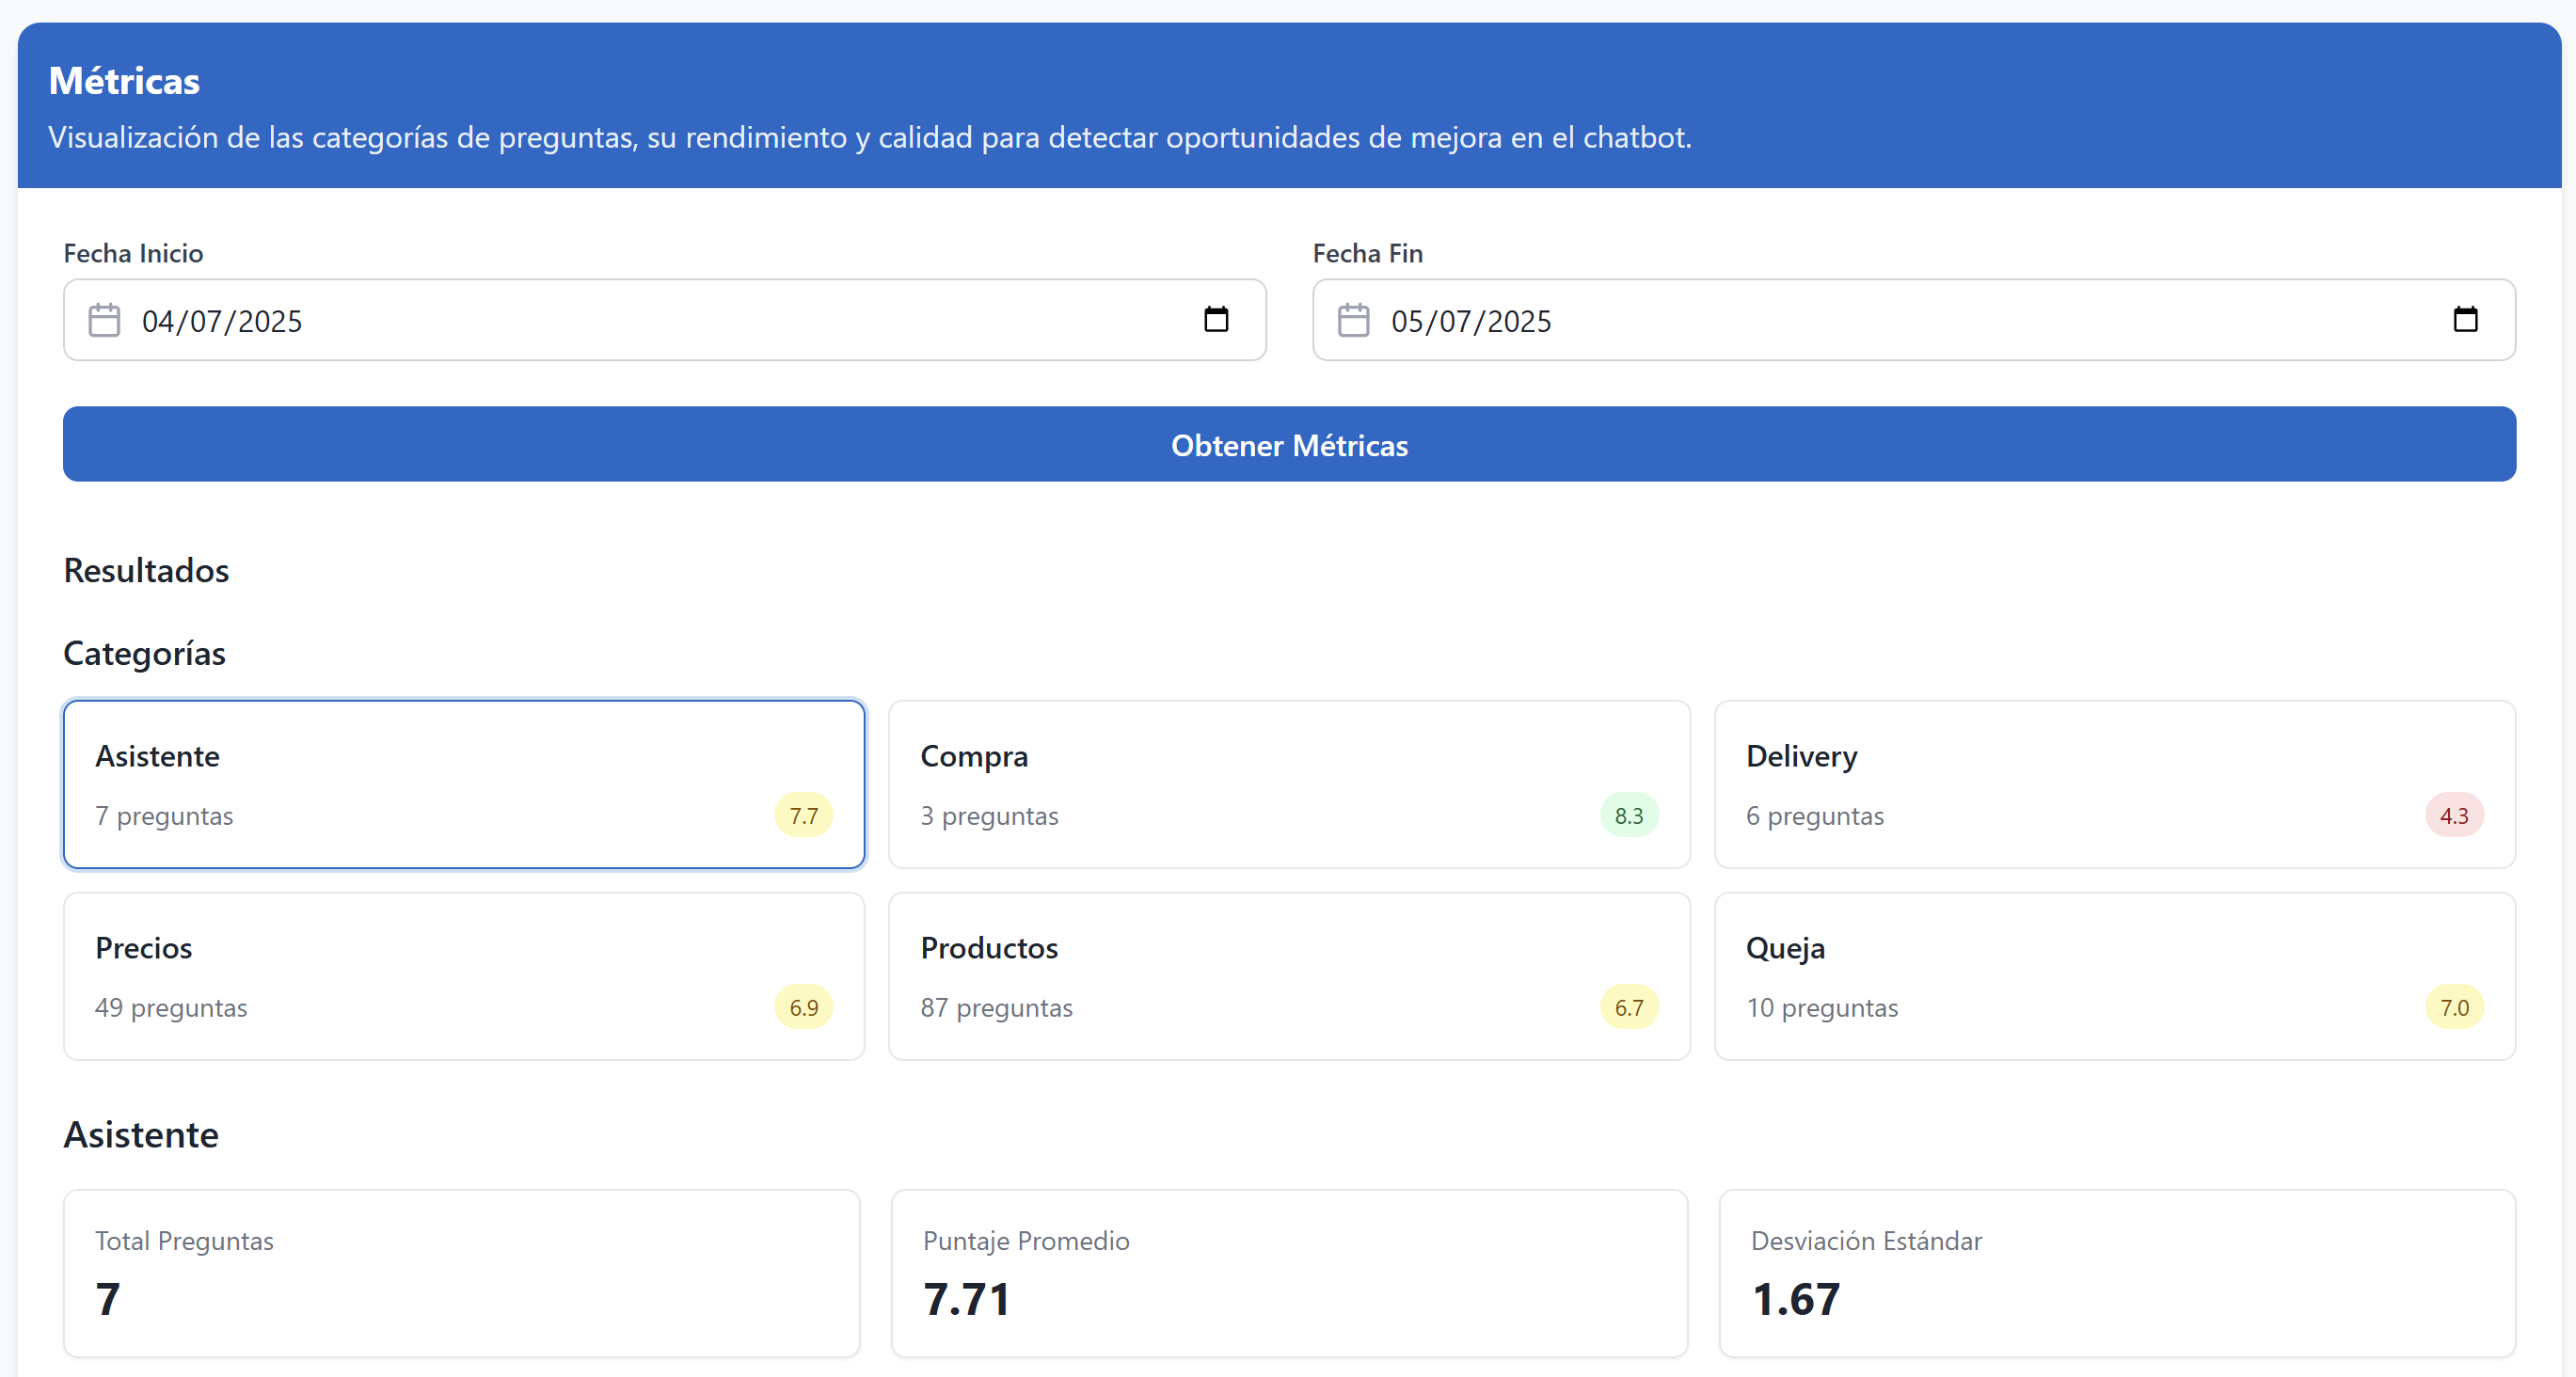
\includegraphics[width=.75\textwidth]{./Figures/metricas1.png}
    \caption{metricas por categoria.}
    \label{fig:objetivos_venn}
  \end{figure}


\begin{lstlisting}[language=Python, caption={Fragmento de código para extracción y evaluación de trazas desde Langfuse}]
for trace in all_traces:
    ...
    if trace.scores and 'Saludo' not in trace.tags:
        score = trace.scores[0]
        traces_df = traces_df.append({...})
\end{lstlisting}




\subsubsection*{Procesamiento y análisis de calidad}

Una vez recolectadas, las trazas se analizan mediante un pipeline estructurado:

\begin{enumerate}
    \item \textbf{Preprocesamiento del texto}: Se normalizan las preguntas (minúsculas, eliminación de acentos y símbolos).
    \item \textbf{Asociación temática}: Se agrupan por etiquetas temáticas estandarizadas.
    \item \textbf{Evaluación cuantitativa}: Se asignan y procesan puntajes de calidad, calculando promedios, desviaciones estándar y clasificando las preguntas como buenas $\geq$ 8, malas < 5, mejores y peores.
    \item \textbf{Agrupamiento semántico}: Se transforman las preguntas en vectores de embeddings y se agrupan con HDBSCAN para detectar redundancias y patrones.
    \item \textbf{Síntesis por grupo}: Se selecciona una pregunta representativa por cada grupo y se genera un resumen por etiqueta temática.
\end{enumerate}

\begin{figure}[htbp]
    \centering
    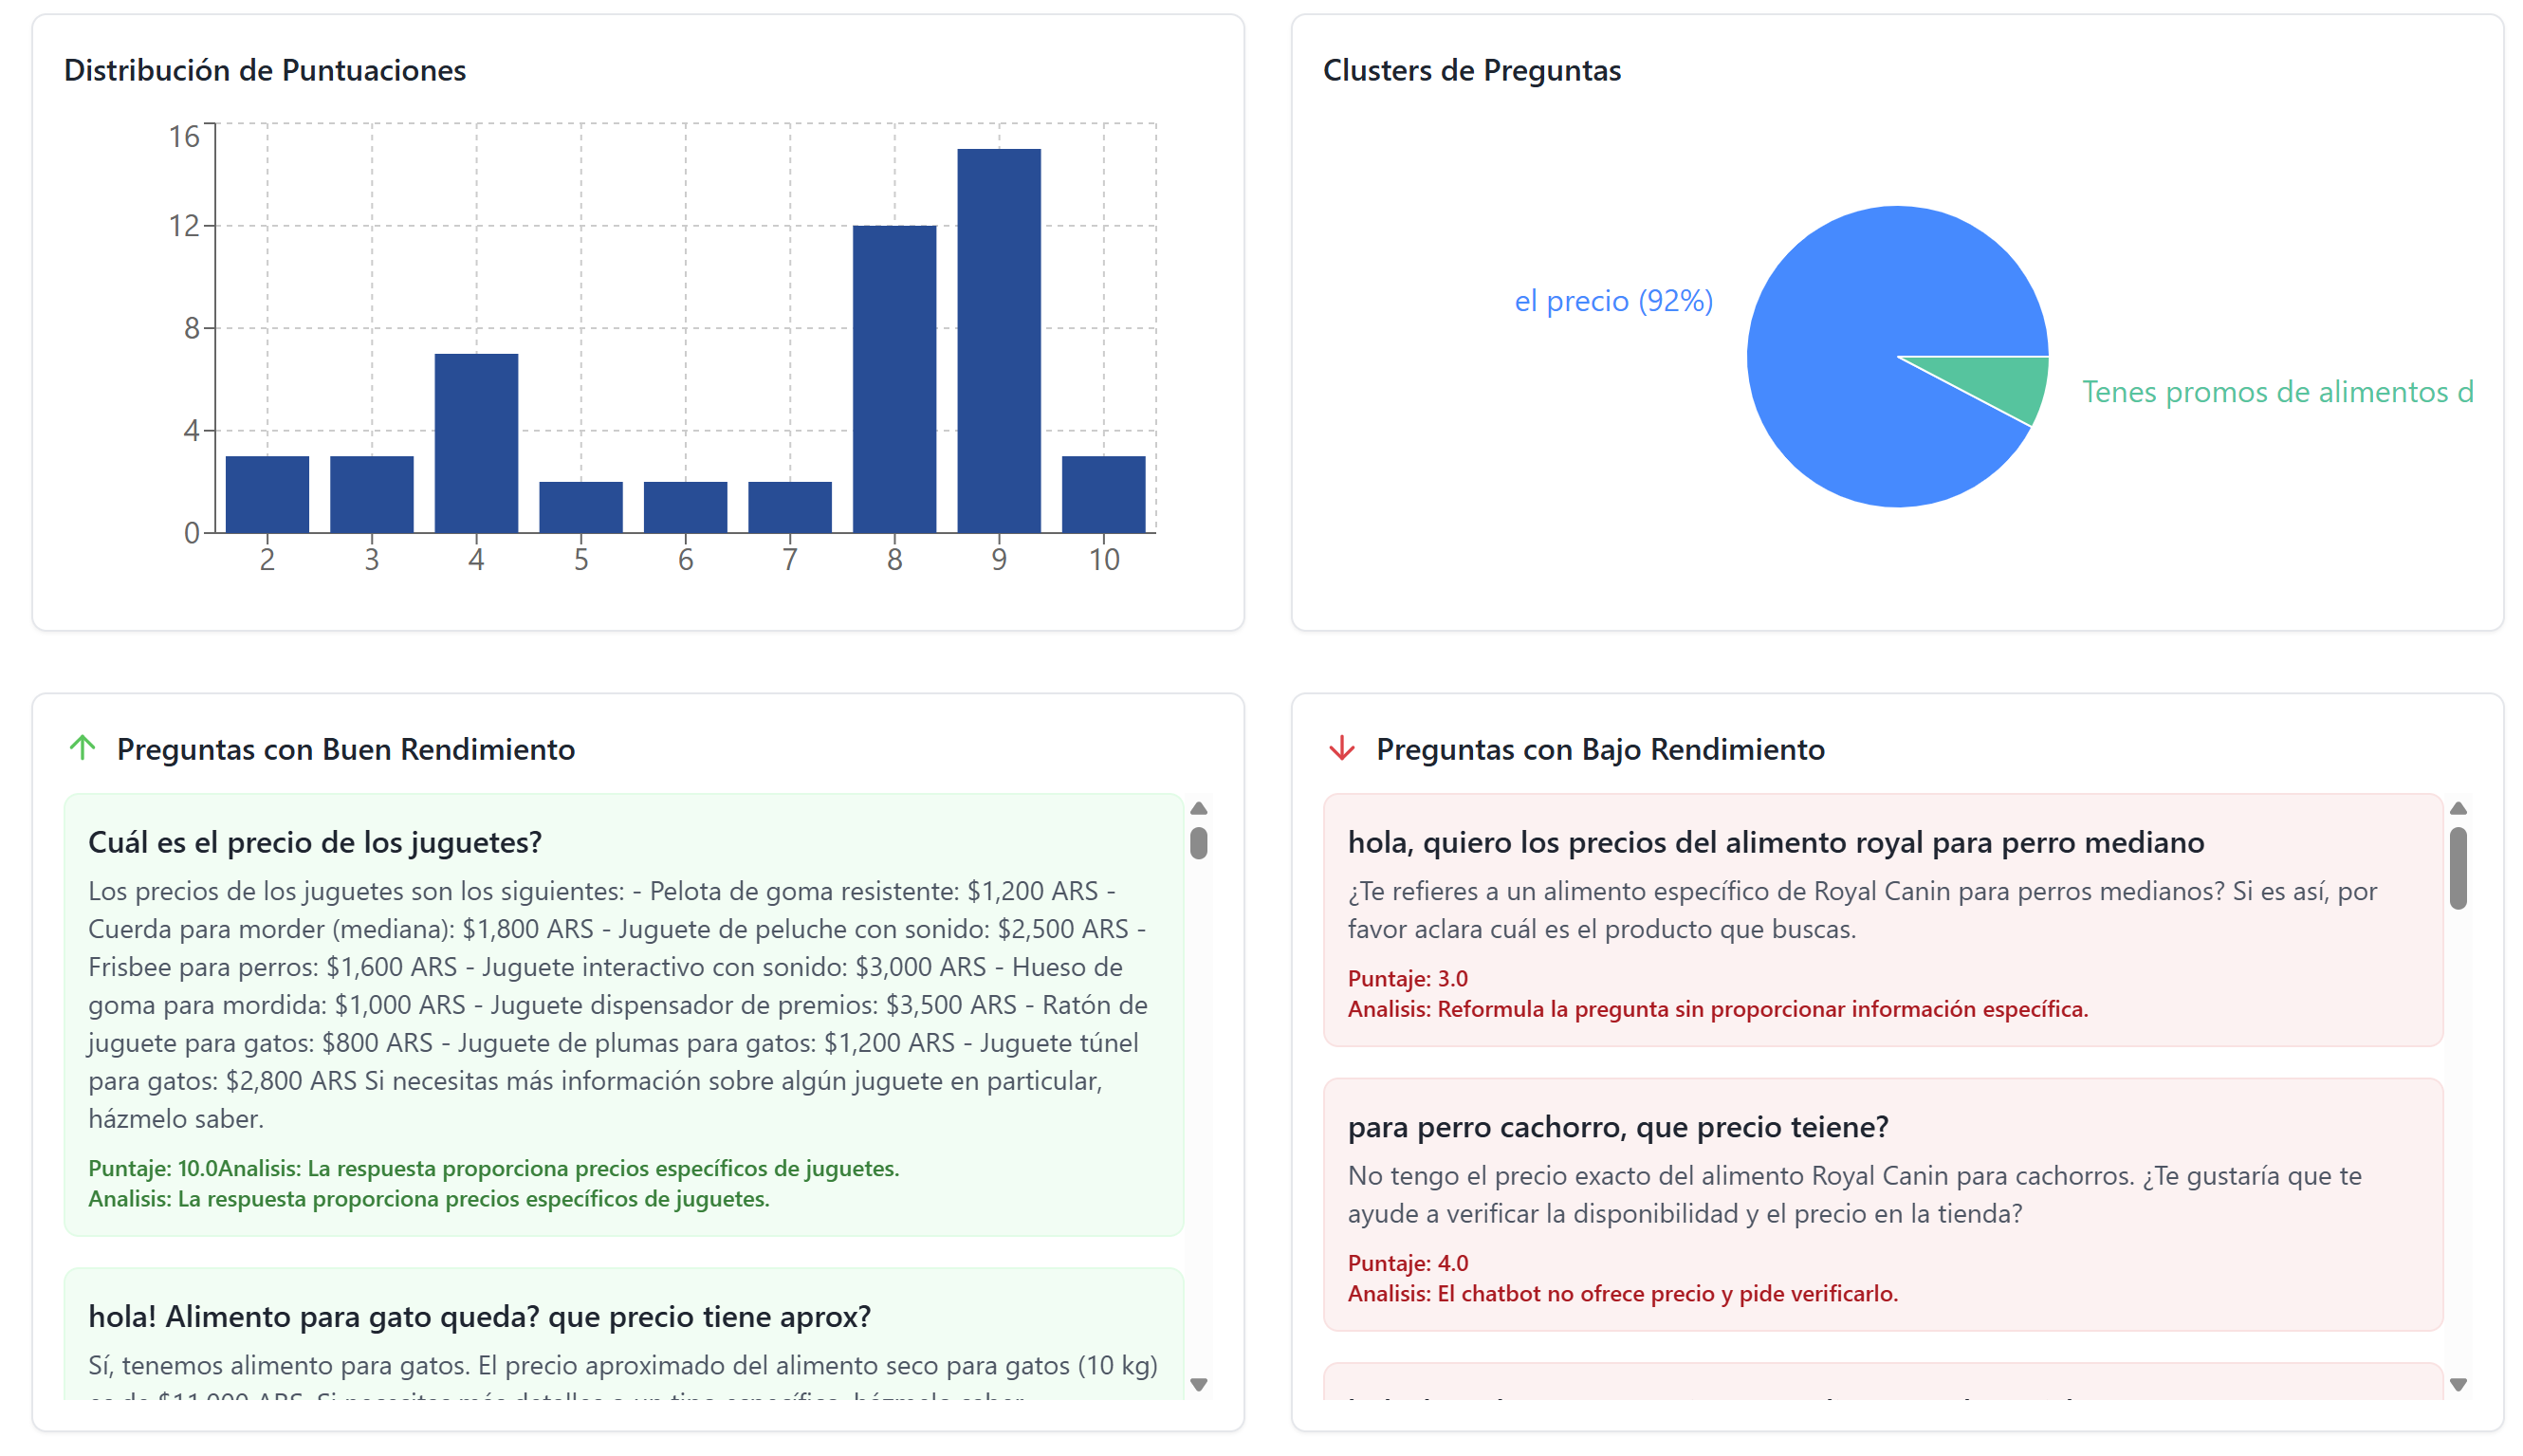
\includegraphics[width=.75\textwidth]{./Figures/metricas2.png}
    \caption{Ejemplo frontend, metricas para preguntas buenas y malas}
    \label{fig:objetivos_venn}
  \end{figure}

Este análisis permite generar reportes automáticos por versión del sistema. Las métricas agregadas permiten evaluar el impacto de cada iteración del sistema. Durante las diferentes versiones, se registraron las siguientes métricas:

\section{Despliegue de la interfaz de pruebas} 

Se implementó una interfaz interactiva mediante \textbf{ReactJS}, diseñada para facilitar tanto pruebas de usuario como análisis administrativo. Esta interfaz permite:

\begin{itemize}
    \item Realizar preguntas al chatbot y visualizar respuestas en tiempo real.
    \item Consultar métricas de evaluación automática y categorías temáticas asignadas a cada pregunta.
    \item Modificar o agregar fragmentos de contexto a través de un formulario de carga.
    \item Acceder a las trazas generadas por Langfuse para cada interacción.
\end{itemize}

\begin{figure}[htbp]
    \centering
    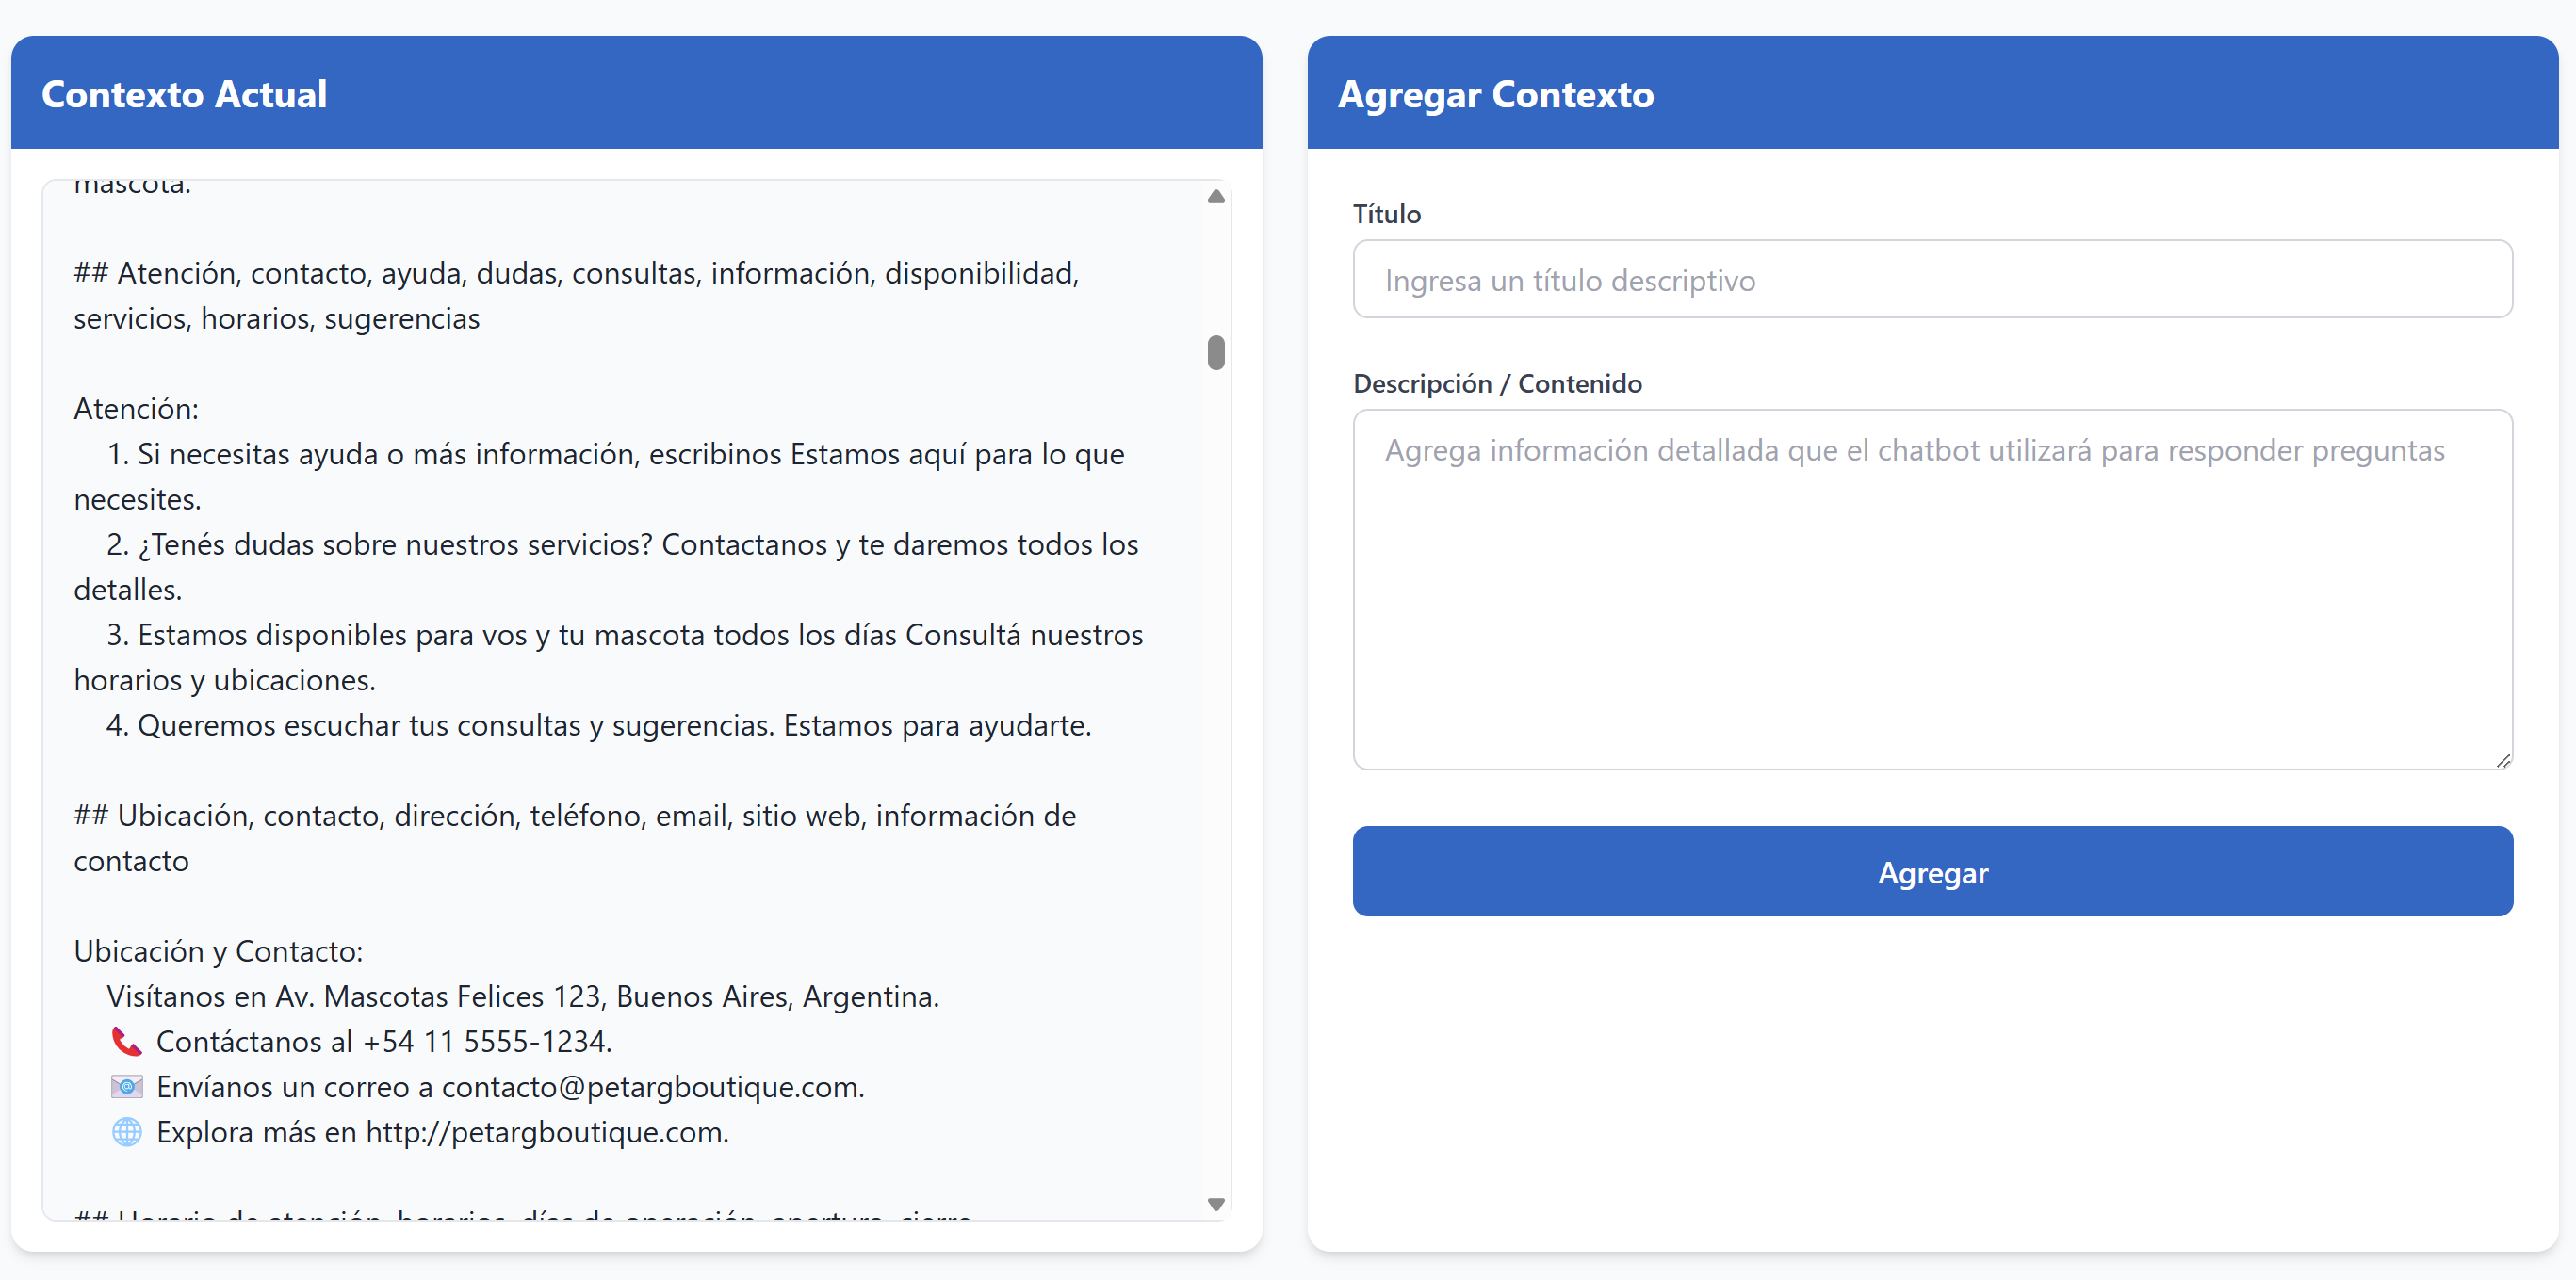
\includegraphics[width=.75\textwidth]{./Figures/contextosui.png}
    \caption{frontend creado para administracion de contextos.}
    \label{fig:objetivos_venn}
  \end{figure}


Está pensada como una herramienta versátil que permite validar mejoras y cambios del sistema en producción de forma inmediata.

